\documentclass[12pt]{report}

% --------------------
% Packages
% --------------------
\usepackage[margin=1in]{geometry}
\usepackage{setspace}
\usepackage{titlesec}
\usepackage{tocloft}
\usepackage{graphicx}
\usepackage{amsmath, amssymb}
\usepackage{caption}
\usepackage{booktabs}
\usepackage{hyperref}

% --------------------
% Spacing
% --------------------
\doublespacing
% --------------------
% Chapter formatting
% --------------------
\titleformat{\chapter}
  {\normalfont\bfseries\Large}
  {\thechapter}
  {1em}
  {}

% --------------------
% Document
% --------------------
\begin{document}

% ====================Thesis Title
% Title Page
% ====================
\begin{titlepage}
\centering
\vspace*{1in}

{\Large \textbf{SAM Based Masking for PIV Experiments}}\\[1.5in]

{\large MIE498Y: Research Thesis}\\[0.5in]

\textbf{Han Hu}\\
1008797553\\[1in]

Supervisor: Prof. Pierre E. Sullivan\\[1in]

Date

\vfill
\end{titlepage}

% ====================
% Front Matter
% ====================
\pagenumbering{roman}

% --------------------
% Abstract (not listed in ToC)
% --------------------
\chapter*{Abstract}
The abstract is generally 100 to 200 words, single-spaced in block form, placed in the centre of a separate page.

\newpage

% --------------------
% Acknowledgements
% --------------------
\chapter*{Acknowledgements}
Acknowledgements (to persons and/or supporting agencies).

\newpage

% --------------------
% Table of Contents
% --------------------
\tableofcontents
\newpage

% --------------------
% List of Symbols
% --------------------
\chapter*{List of Symbols}

\begin{tabular}{ll}
Symbol & Definition \\
\hline
$A$ & Example symbol \\
$B$ & Example definition \\
\end{tabular}

\newpage

% --------------------
% List of Figures
% --------------------
\listoffigures
\newpage

% --------------------
% List of Tables
% --------------------
\listoftables
\newpage

% ====================
% Main Thesis
% ====================
\pagenumbering{arabic}

\chapter{Introduction}
\section{Particle Image Velocimetry (PIV)}
Particle Imagery Velocimetry (PIV) is a flow visualization technique that measures the instantaneous 
velocity of the fluid flow by calculating the displacement of laser illuminated particles in two different 
images taken, this is also known as the an image pair in the context of PIV experiments. 
In PIV experiments, small particles are seeded into the fluid flow, and photos will be taken for those
particles as they became illuminated by laser. By comparing the displacement of the particles seen from the image
pair and assuming that the motion of particles follows the motion of the fluid, the fluid velocity field can be calculated.
\section{PIV Masking}
The use of laser in the experiment resulted in measurement errors near object boundaries 
due to the reflection from the object. To resolve this issue, masks are created to exclude certain 
areas from the solution algorithm. Traditionally, manual masking is performed by researchers to define zones of 
exclusion. However, such method is impractical for measurement of moving objects as the experiment 
usually uses high speed camera and has a significant amount of data needing labeling. Some automated 
masking procedures are developed to help with these scenario. One of them involves fitting predetermined 
polynomial to the PIV data as the output mask. However this method requires preexisting knowledge about 
the motion and shape of the object measured, which would be impractical in some cases.
\section{Computer Vision}
Computer vision is a sub-field of artificial intelligence which focused on enabling machines and algorithms to 
interpretate visual data, usually in the form of images or videos. The origin of computer vision can be traced back
to the 1960s. Today computer vision is used for a range of tasks, from image denoising to segmentation and object labeling.

\section{Computer Vision for PIV}
Computer vision has been proposed as a measure for mask generation in PIV experiments. The proposed algorithm 
uses the Segment Anything Model developed by Meta AI capable of zero-shot generalization, to create masks 
around bounding points determined by the Grounding-Dino model, capable of identifying location of objects 
using natural language input. This inherently simplifies the workflow of the masking procedure and provides 
alternative measure to masking objects in motion in PIV experiments. This paper analyzes the aforementioned computer vision algorithm used in PIV experiment by adapting 
it to a python based PIV solver. The output from the modified solver will then be validated against 
manual masking and polynomial fitting to obtain the final conclusion regarding the feasibility of using 
computer vision for PIV experiments.

\chapter{Literature Review}
This chapter introduces coding libraries and literature critical to the research discussed in this report.
\section{OpenPIV}
OpenPIV is an open-source, community driven project on the development of a free PIV analysis
and post-processing software. The python version of the package, OpenPIV-Python is currently 
available throught the Python Package Index (PyPI). This package offered flexible and easy to use interface
for the processing of PIV data in the form of image pairs. The package is available both in the code format
and in the GUI format for both windows and linux platforms.

The OpenPIV library provides access to correlation algorithm essential to the computation of velocity fields,
and validation through calculation which is studied in this report. Due to the noisy nature of the immediate object
boundary of objects embedded in flow as a result of reflection. The signal to noise ratio validation is of specific interest to 
the subject of study in this report. This library provides the method to analyze the efficiency of the masks identified by the computer vision
algorithms by investigating the effect if has on removing significantly noisy layers immediate to object boundaries. 

\section{OpenPIV-Python-CPU}
OpenPIV-Python-CPU is a library developed from the code of OpenPIV-Python and optimized for the perfomrance when the
software is ran on the Central Processing Unit (CPU). While similar to the OpenPIV-Pyhton code from many aspects, this
library uses different correlation algorithm and interogation windows sizing in hopes of improved performance. The database uses
a different but similar syntax for its operation compared to the OpenPIV-Python module. While providing simplifications to the model, this model
is shown to construct the fluid velocity profile to a satisfactory degree. This model also provides signal to noise validation that is critical for
the validation step of this research.

This module will be used as the main algorithm for the computation of PIV data for the aforementioned reasons and the availability of tutorials in the form
of jupyter notebooks. The code used for this research are modified on the basis of those tutorials as they provide a proven workflow for PIV analysis.
The mask generation step will be inserted into the PIV tutorials and the validation step will be slightly isolated for the 
purpose of this research. This is to isolate and show the difference or indifference of the analysis results to analyze the validity of using computer vision to generate
masks for PIV experiments.
\section{Zero Shot Learning}
Zero shot learning refer to the attempt to classify instances to classes with no previously labeled instances. Countrary
to supervised learning, which requires labeling training data with classes for those classes to be used in classification.
While recent advancements in supervised learning provides more and more powerful models for classification, the concept 
itself sufferes from inherent shotcomings such as the inability to work with rare classifications or cases where obtaining data 
under a certain class is prohibitively expensive. For these reasons, Zero shot learning has been proposed and since its debut, this method has
received high attentiondue to the uniqueness it have on the concept of deep learning algorithms. This research uses models considered to be in the realms
of zero shot learning to recognize the expensiveness of obtainnig labeled data in fluid dynamics research.
\section{Segment Anything Model (SAM) NEED WORK FIGURE WAITING FOR CHANGE}
The Segment Anything Model (SAM) developed by Meta AI is used in this project. The model is built to be capable of zero-shot generalization, where 
it can recognize different objects from an image without further training for the specific use case.
The SAM model takes a photo and points indicating the location of the desired object as input to generate a mask. The model is available 
both online as a demo and as source code which this research benefits from. Figure \ref{fig:SAMIntro} attached below shows the application of SAM in the online demo
to generate a mask on one of the PIV images used for this research. Notice how the model was able to recognize the shape of the airfoil when a hollow point
is placed on the airfoil. SAM is used as the main model to create the mask once the location of the input box is identified through the use of other 
machine learning models.

\begin{figure}[htbp] % [htbp] helps position the figure
    \centering
    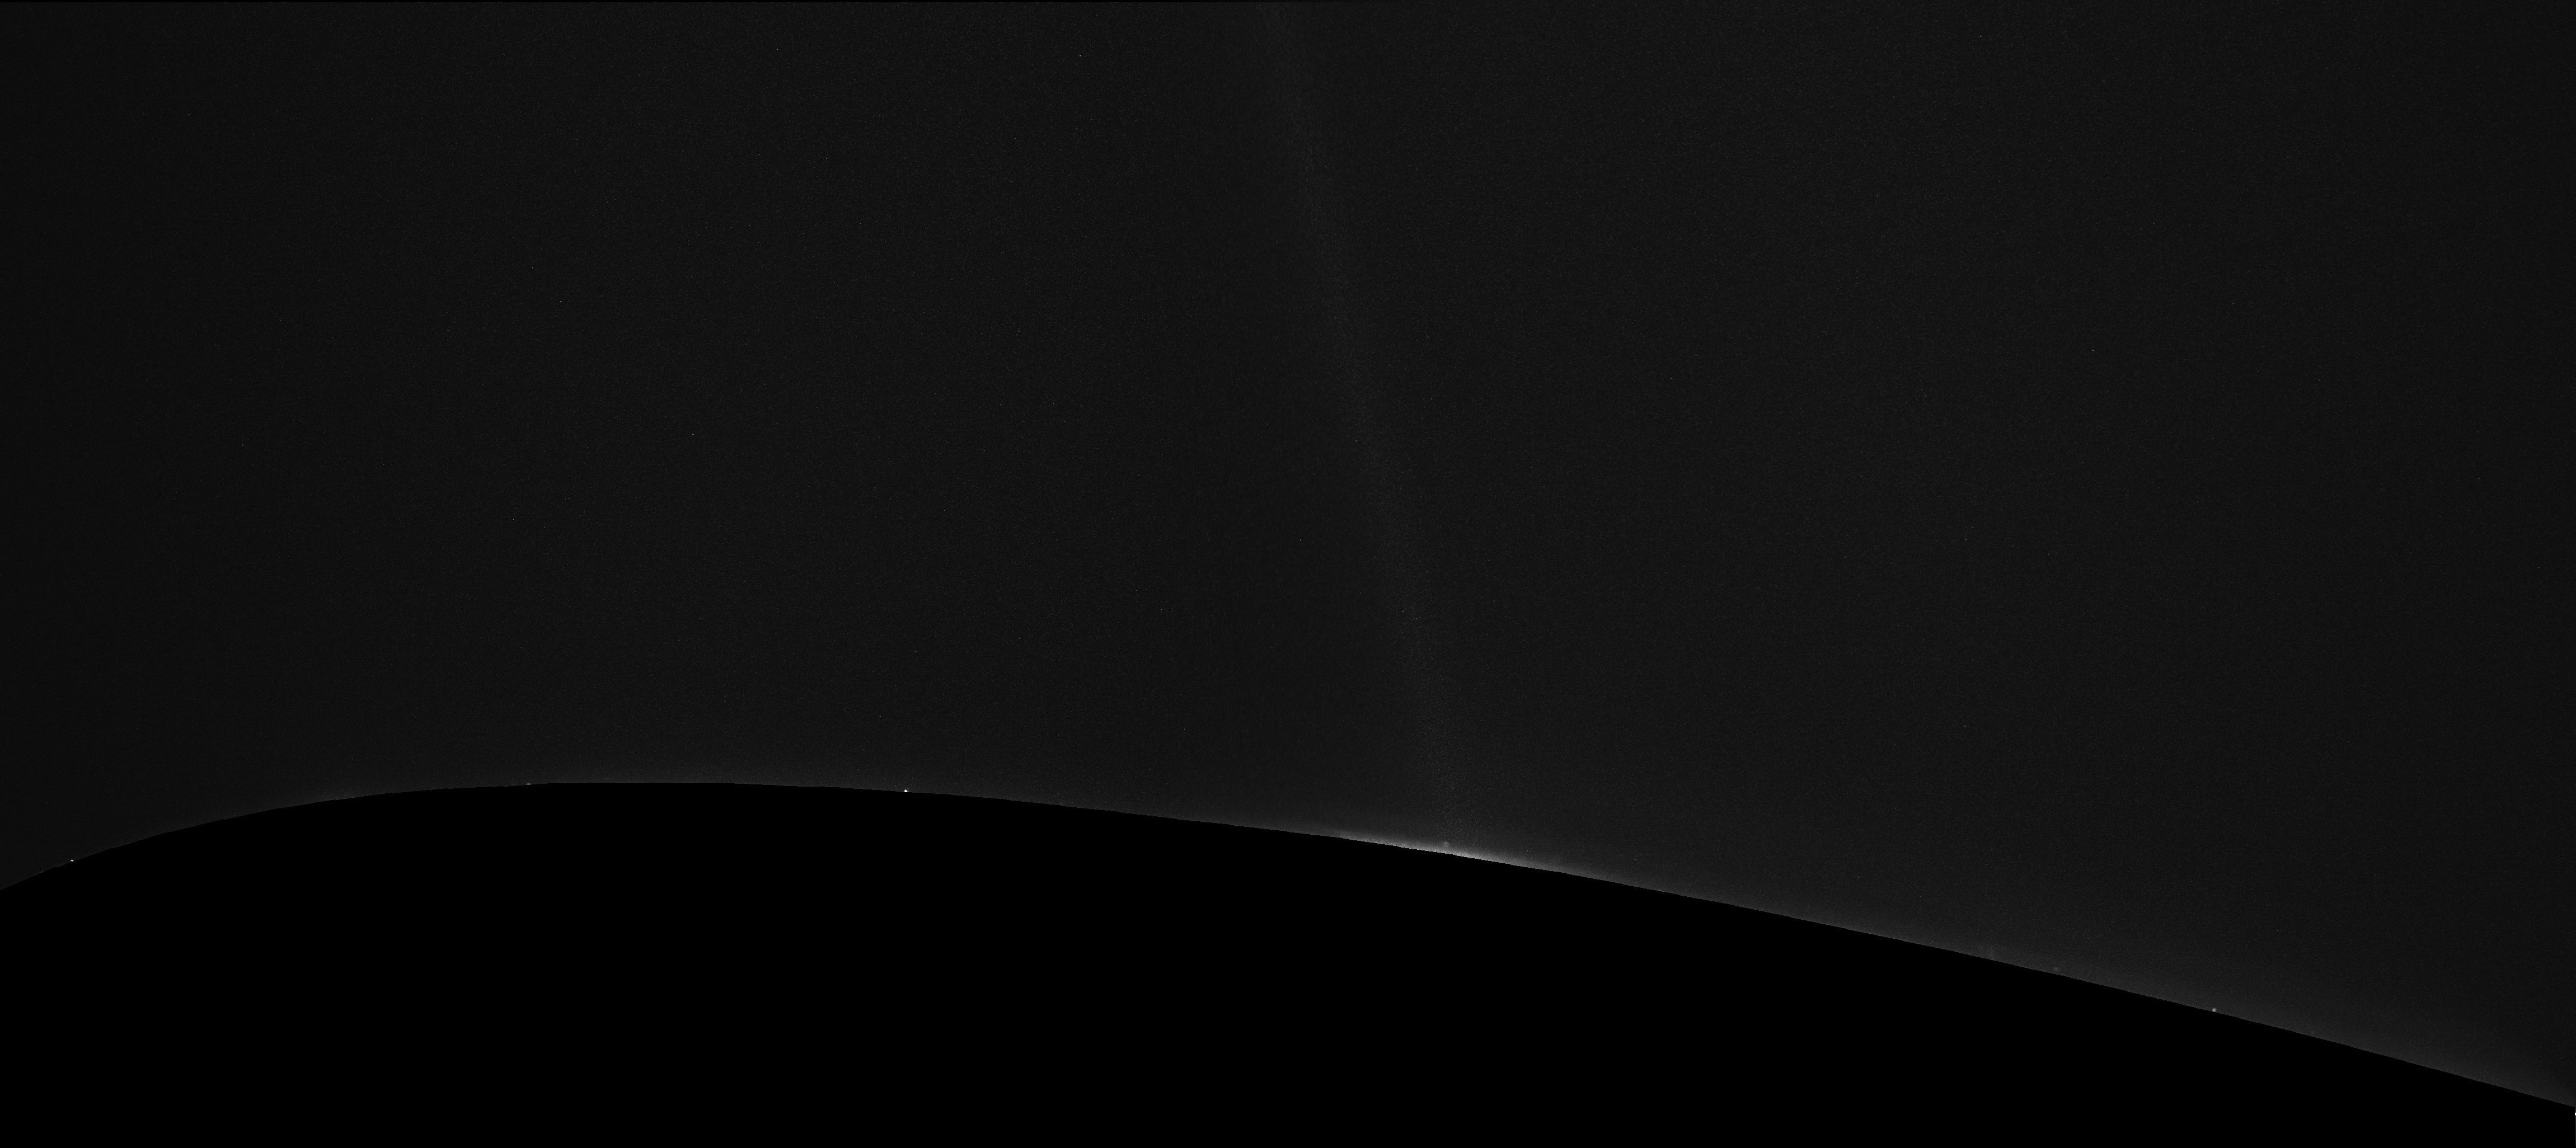
\includegraphics[width=0.75\textwidth]{./Figures/SAMDemo.png} % Resize and name
    \caption{PIV Experiment Data: Raw Image (left); Labeled and Masked (right).}
    \label{fig:SAMIntro}
\end{figure}

Two models are evaluated in this report to study the masking capabilities and efficiency of the previous generation of SAM and
the current generation of SAM. In the first generation of SAM, due to the inability to take natural language input, additional
models are employed to supply SAM with input points. The used model is the GroundingDINO model. The later model, SAM3 has the built in capability to take
natural language input, therefore the GroundingDINO module is not used with SAM3.

\section{Grounding Dino}
Grounding Dino is the 
\section{Masking by Polynomial Fitting}
\section{Flow Segmentation Using SAM}


\chapter{Methodology}
Describe how the work was conducted.
\section{Programming Environment Setup}
\section{Code Preparation and Changes Made}
\section{Validation}
\subsection{Mask Size}
\subsection{Signal to Noise Ratio}
\subsection{Median Tolerances}


\chapter{Results}
Present results and findings.

\chapter{Discussion}
Interpretation and discussion of results.

\chapter{Conclusions}
Summary of findings and conclusions.

% ====================
% References
% ====================
\chapter*{References}
\addcontentsline{toc}{chapter}{References}

% ====================
% Appendices
% ====================
\appendix

\chapter{Appendix A}
Begin each appendix on a separate page and label each as Appendix A, Appendix B, etc.

\chapter{Appendix B}
Additional material.

\end{document}